\documentclass[ngerman,a4paper,order=firstname]{../../texmf/tex/latex/mathscript/mathscript}
\usepackage{../../texmf/tex/latex/mathoperators/mathoperators}

\title{\textbf{Algebra und Zahlentheorie SS 2019}}
\author{Dozent: Prof. Dr. \person{Arno Fehm}}

\begin{document}
\pagenumbering{roman}
\pagestyle{plain}

\maketitle

\hypertarget{tocpage}{}
\tableofcontents
\bookmark[dest=tocpage,level=1]{Inhaltsverzeichnis}

\pagebreak
\pagenumbering{arabic}
\pagestyle{fancy}

\chapter*{Vorwort}
Schön, dass du unser Skript für die Vorlesung \textit{Lineare Algebra und analytische Geometrie 1} bei Prof. Dr. Arno Fehm im WS2017/18 gefunden hast! \footnote{Obwohl man sagen kann, dass es in dieser Vorlesung nur um Lineare Algebra ging, der Teil mit der analytischen Geometrie wurde vernachlässigt. Liegt wahrscheinlich auch daran, dass es demnächst eine Reform der Studienordnung gibt, in der aus der Vorlesung \textit{Lineare Algebra und analytische Geometrie} die Vorlesung \textit{Einführung in die Lineare Algebra} wird.}

Wir verwalten dieses Skript mittels Github \footnote{Github ist eine Seite, mit der man Quelltext online verwalten kann. Dies ist dahingehend ganz nützlich, dass man die Quelltext-Dateien relativ einfach miteinander synchronisieren kann, wenn man mit mehren Leuten an einem Projekt arbeitet.}, d.h. du findest den gesamten \LaTeX-Quelltext auf \url{https://github.com/henrydatei/TUD_MATH_BA}. Unser Ziel ist, für alle Pflichtveranstaltungen von \textit{Mathematik-Bachelor} ein gut lesbares Skript anzubieten. Für die Programme, die in den Übungen zur Vorlesung \textit{Programmieren für Mathematiker} geschrieben werden sollen, habe ich ein eigenes Repository eingerichtet; es findet sich bei \url{https://github.com/henrydatei/TU_PROG}.

Du kannst dir gerne dort die \LaTeX-Quelldateien herunterladen, die Dateien für exakt dieses Skript sind im Ordner \texttt{1. Semester/LAAG ueberarbeitet}. Es lohnt sich auf jeden Fall während des Studiums die Skriptsprache \LaTeX{} zu lernen, denn Dokumente, die viele mathematische oder physikalische Formeln enthalten, lassen sich sehr gut mittels \LaTeX{} darstellen, in Word oder anderen Office-Programmen sieht so etwas dann eher dürftig aus.

\LaTeX{} zu lernen ist gar nicht so schwierig, ich habe dafür am Anfang des ersten Semesters wenige Wochen benötigt, dann kannte ich die wichtigsten Befehle und konnte den Vorgänger dieses Skriptes schreiben (\texttt{1. Semester/LAAG}, Vorsicht: hässlich, aber der Quelltext ist relativ gut verständlich).

Es sei an dieser Stelle darauf hingewiesen (wie in jedem anderem Skript auch \smiley{}), dass dieses Skript nicht den Besuch der Vorlesungen ersetzen kann. Es könnte sein, dass Prof. Fehm seine Vorlesung immer mal wieder an die Studenten anpasst; wahrscheinlich immer dann, wenn die Prüfungsergebnisse zu schlecht waren. Nichtsdestotrotz veröffentlicht Prof. Fehm sein Skript auf seiner Homepage \url{http://www.math.tu-dresden.de/~afehm/lehre.html}. Allerdings ist dieses Skript recht hässlich, besonders was die Übersichtlichkeit angeht.

Wir möchten deswegen ein Skript bereitstellen, dass zum einen übersichtlich ist, zum anderen \textit{alle} Inhalt aus der Vorlesung enthält, das sind insbesondere Diagramme, die sich nicht im offiziellen Skript befinden, aber das Verständnis des Inhalts deutlich erleichtern. Ich denke, dass uns dies erfolgreich gelungen ist.

Trotz intensivem Korrekturlesen können sich immer noch Fehler in diesem Skript befinden. Es wäre deswegen ganz toll von dir, wenn du auf unserer Github-Seite \url{https://github.com/henrydatei/TUD_MATH_BA} ein neues Issue erstellst und damit auch anderen hilfst, dass dieses Skript immer besser wird.
\chapter*{Motivation und Einführung}
%TODO
\chapter{Körper}
\section{Körpererweiterungen}

Sei $K,L,M$ Körper.

\begin{remark}
	In diesem Kapitel bedeutet ``Ring'' \emph{immer} kommutativer Ring mit Einselement, und ein Ringhomomorphismus bildet stets das Einselement auf das Einselement ab.
	Insbesondere gibt es für jeden Ring einen eindeutig bestimmten Ringhomomorphismus $: \Z \to R$.
\end{remark}

\begin{remark}
	\proplbl{1_1_2}
	\begin{enumerate}[label=(\alph*)]
		\item Ein \emph{Körper} ist ein Ring $R$, in dem eine der folgenden äquivalenten bedingungen gilt:
		\begin{enumerate}[label=\arabic*)]
			\item $0 \neq 1$ und jedes $0 \neq x \in R$ ist invertierbar
			\item $R^{\times} = R \setminus \set{0}$
			\item $R$ hat genau zwei Hauptideale (nämlich $(0)$ und $(1)$)
			\item $(0)$ ist ein maximales Ideal von $R$
			\item $(0)$ ist das einzige echte Ideal von $R$
			\item $(0)$ ist das einzigste Primideal von $R$
		\end{enumerate}
		\item Insbesondere sind Körper \emph{nullteilerfrei}, weshalb $\Ker(\Z \to K)$ prim ist.
		\item Aus (5) folgt: Jeder Ringhomomorphismus $K \to L$ ist injektiv %TODO add ref to (5) and check the ringhomo!
		\item Der Durchschnitt einer Familie von Teilkörpern von $K$ ist wieder ein Teilkörper von $K$.
	\end{enumerate}
\end{remark}

\begin{definition}[Charakteristik]
	Die \begriff{Charakteristik} von $K$, $\chara(K)$, ist das $p \in \set{0,2,3,5,7, \dots}$ mit $\Ker(\Z \to K) = (p)$.
\end{definition}

\begin{example}
	\proplbl{1_1_4}
	\begin{enumerate}
		\item $\chara(\Q) = 0$ und $\chara(\Fp) = (p)$ ($p =$ Primzahl), wobei $\Fp = \lnkset{\Z}{p\Z}$
		\item Ist $K_0 \subseteq K$ Teilkörper, so ist $\chara(K_0) = \chara(K)$.
	\end{enumerate}
\end{example}

\begin{definition}[Primkörper]
	Der \begriff{Primkörper} von $K$ ist der kleinste Teilkörper von $K$. (existiert nach \propref{1_1_2}(d)) %TODO add ref!
\end{definition}

\begin{proposition}
	Sei $\field$ der Primkörper von $K$.
	\begin{enumerate}[label=(\alph*)]
		\item $\chara(K)  = 0 \Leftrightarrow \field \cong \Q$
		\item $\chara(K)  = p > 0 \Leftrightarrow \field \cong \Fp$
	\end{enumerate}
\end{proposition}

\begin{proof}
	``$\Leftarrow$'': \propref{1_1_4}\\ % (beide?)
	``$\Rightarrow$'': $\Image(\Z \to K) \subseteq \field$ und $\Image(\Z \to K) \cong \lnkset{\Z}{\Ker(\Z \to K)}$
	\begin{enumerate}[label=(\alph*)]
		\item $\Image(\Z \to K) \cong \lnkset{Z}{(0)} \cong \Z \Rightarrow \field = \Quot(\Image(\Z \to K)) \cong \Quot(\Z) \cong \Q$
		\item $\Image(\Z \to K) \cong \lnkset{Z}{(p)} \cong \Fp$ ist Teilkörper von K $\Rightarrow \field = \Image(\Z \to K) \cong \Fp$
	\end{enumerate}
\end{proof}

\begin{definition}[Körpererweiterung]
	Ist $K$ ein Teilkörper von $L$, so nennt man $L$ eine \begriff{Köpererweiterung} von $K$, auch geschrieben $L\vert K$.
\end{definition}

\begin{definition}[$K$-Homomorphismus]
	Seien $L_1\vert K$ und $L_2 \vert K$ Körpererweiterungen.
	\begin{enumerate}
		\item Ein Ringhomomorphismus $\phi\colon L_1 \to L_2$ ist ein $K$-Homomorphismus, wenn $\phi\vert_K = \id_K$ (i.Z. $\phi: L_1 \to L_2$)
		\item $\Hom_K(L_1,L_2) = \set{\phi \mid \phi: L_1 \to L_2 \text{ ist $K$-Homomorphismus}}$
		\item $L_1$ und $L_2$ sind $K$-isomorph (i.Z. $L_1 \cong L_2$), wenn es einen Isomorphismus: $\phi \in \Hom_K(L_1, L_2)$ gibt.
	\end{enumerate}
\end{definition}

\begin{remark}
	$L\vert K$ eine Körpererweiterung, so wird $L$ durch Einschränkung der Multiplikation zu einem $K$-Vektorraum.
\end{remark}

\begin{definition}[Körpergrad]
	$[L:K]:= \dim_k(L) \in \N \cup \{\infty\}$, der \begriff{Körpergrad} der Körpererweiterungen $L\vert K$.
\end{definition}

\begin{example}
	\begin{enumerate}[label=(\alph*)]
		\item $[K: K] = 1$
		\item $[\C:\R] = 2$ (Basis $(1,i)$) (aber $(\C:\R) = \infty$)
		\item $[\R:\Q] = \infty$ (mit Abzählarbarkeitsargument oder siehe §2) %TODO ref later, when we are in chap 2!
		\item $[K(x):K] = \infty$ ($K(x) = \Quot(K[x])$ (vgl. GEO II.8)
	\end{enumerate}
\end{example}

\begin{proposition}
	Für $K \subseteq L \subseteq M$ Körper ist $[M:K] = [M:L]\cdot [L:K]$ \\
	(``Körpergrad ist multiplikativ'')
\end{proposition}

\begin{proof} %TODO maybe make unnumbered lemma here for the claim?
	Behauptung: Sei $x_1, \dots, x_n \in L$ $K$-linear unabhängig und $y_1, \dots, y_m \in M$ $L$-linear unabhängig\\
	$\Rightarrow x_i y_j, i \in \set{1,\dots,n}, j \in \set{1, \dots, m}$ $K$-linear unabhängig.\\
	Beweis: $\sum_{i,j} \lambda_{ij}x_i y_j = 0$ mit $\lambda_{ij} \in K$\\
	$\Rightarrow \sum_{j}\underbrace{\left( \sum_{i} \lambda_{ij}x_i \right)}_{\in L}y_j = 0 
	\xRightarrow{y_j L\text{-l.u.}} \sum_{i} \lambda_{ij} x_i = 0\quad\forall j
	\xRightarrow{y_j K\text{-l.u.}} \lambda_{ij} = 0\quad\forall i, \forall j$
	\begin{itemize}
		\item $[L:K] = \infty$ oder $[M:L] = \infty \Rightarrow [M:K] = \infty$
		\item $[L:K] = n, [M:L] = m < \infty$\\
		$(x_1, \dots, x_n)$ Basis des $K$-Vektorraum $L$ und $(y_1, \dots, y_m)$ Basis des $L$-Vektorraums M\\
		$\Rightarrow \set{x_i y_j \colon i = 1, \dots, n; j = 1, \dots, m}$ $K$-linear unabhängig und \\
		$\sum_{i,j} Kx_i y_j = \sum_{j}\left( \sum_{i} \lambda_{ij}x_i \right)y_j = M$, also ist \\
		$\set{x_i y_j \colon i = 1, \dots ,n; j = 1, \dots, m}$ Basis von $M$ 
	\end{itemize}
\end{proof}

\begin{definition}[Körpergrad endlich]
	$L\vert K$ endlich $:\Leftrightarrow [L:K] < \infty$.
\end{definition}

%%%%%%%%%%%%%%%%%%%%%%%%%%%% 2nd lecture %%%%%%%%%%%%%%%%%%%%%%%%%%%%%%%%%%%%%%%%%%%%%%%%%%%%%%

\begin{definition}[Unterring, Teilkörper]
	Sei $L\vert K$ eine Körpererweiterung $a_1, a_2, \dots, a_n \in L$.
	\begin{enumerate}
		\item $K[a_1, \dots, a_n]$ ist kleinster \begriff{Unterring} von $L$, der $K \cup \set{a_1, \dots, a_n}$ enthält (``$a_1, \dots, a_n$ über $K$ erzeugt'')
		\item $K[a_1, \dots, a_n]$ ist kleinster \begriff{Teilkörper} von $L$, der $K \cup \set{a_1, \dots, a_n}$ enthält (``von ``$a_1, \dots, a_n$ über $K$ erzeugte'', ``$a_1, \dots, a_n$'' zu $K$ adjungieren)
		\item $L | K$ ist \begriff{endlich erzeugt} $:\Leftrightarrow a_1, \dots , a_n \in L : L=K(a_1, \dots, a_n)$
		\item $L | K$ ist \begriff{einfach} $:\Leftrightarrow$ existiert $a \in L: L=K(a)$  
	\end{enumerate}
\end{definition}

\begin{remark}
	\proplbl{1_1_15}
	\begin{enumerate}[label=(\alph*)]
		\item $L\vert K$ endlich $\Rightarrow L\vert K$ endlich erzeugt.
		\item $K[a_1, \dots, a_n]$ ist das Bild des Homomorphismus
		\begin{align}
		\begin{cases}
		K[x_1, \dots, x_n] &\to L\\
		f &\mapsto f(a_1, \dots, a_n)
		\end{cases}\notag
		\end{align}
		und $K(a_1, \dots , a_n) = \set{\alpha \beta \colon \alpha, \beta \in K[a_1, \dots, a_n], \beta \neq 0} \cong \Quot(K[a_1, \dots, a_n])$
	\end{enumerate}
\end{remark}
\section{Algebraische Körpererweiterungen}

Sei $L \vert K$ eine Körpererweiterung.

\begin{definition}[algebraisch, transzendent]
	Sei $\alpha \in L$. Gibt es ein $0 \neq f \in K$ mit $f(\alpha) = 0$, so heißt $\alpha$ \begriff{algebraisch} über $K$, andernfalls \begriff{transzendent} über $K$.
\end{definition}

\begin{example}
	\begin{enumerate}[label=(\alph*)]
		\item $\alpha \in K \Rightarrow \alpha$ ist algebraisch über $K$ (denn $f(\alpha) = 0$ für $f = X - \alpha \in K$)
		\item $\sqrt{-1} \in \Q(\sqrt{-1})$ ist algebraisch über $\Q$ (denn $f(\sqrt{-1})=0$ für $f = X^2 + 1 \in \Q$) \\
		$\sqrt{-1} \in \C$ ist algebraisch über $\R$        
	\end{enumerate}
\end{example}

\begin{remark}
	\proplbl{1_2_3}
	Sind $K \subseteq L \subseteq M$ Körper und $\alpha \in M$ algebraisch über $K$, so auch über $L$.
\end{remark}

\begin{lemma} 
	\proplbl{1_2_4}
	Genau dann ist $\alpha \in L$ algebraisch über $K$, wenn $1, \alpha, \alpha^2 , \dots$ $K$-linear abhängig sind.
\end{lemma}

\begin{proof}
	Für $\lambda_0 , \lambda_1 , \dots \in K$, fast alle gleich Null, so ist
	\begin{align}
	\sum_{i=0}^\infty \lambda_i \alpha^i :\Leftrightarrow f(\alpha) = 0 \text{ für } f = \sum_{i=0}^\infty \lambda_i X^i \in K\notag
	\end{align}
\end{proof}

\begin{lemma}
	Betrachte den Epimorphismus
	\begin{align}
	\phi_{\alpha}:\begin{cases}
	K[x] &\to K[\alpha]\\
	f &\mapsto f(\alpha).
	\end{cases}\notag
	\end{align}
	Genau dann ist $\alpha$ algebraisch über $K$, wenn $\Ker(\phi_\alpha) \neq (0)$. In diesem Fall ist $\Ker(\phi_\alpha) = (f_\alpha)$ mit einem eindeutig bestimmten irreduziblen, normierten $f_\alpha \in K$.
\end{lemma}

\begin{proof}
	$K$ Hauptidealring $\Rightarrow \Ker(\phi_\alpha) = (f_\alpha)$, $f_\alpha \in K$, o.E. sei $f_{\alpha}$ normiert. Aus $K[\alpha] \subseteq L$ nullteilerfrei folgt, dass $\Ker(\phi_\alpha)$ prim ist. Somit ist $f_\alpha$ prim und im Hauptidealring also auch irreduzibel.
\end{proof}

\begin{definition}[Monimalpolynom, Grad]
	Sei $\alpha \in L$ algebraisch über $K$, $\Ker(\phi_\alpha) = (f_\alpha)$ mit $f_\alpha \in K$ normiert und irreduzibel.
	\begin{enumerate}
		\item $\MinPol(\alpha\vert K)  f_\alpha$, das \begriff{Minimalpolynom} von $\alpha$ über $K$.
		\item $\deg(\alpha\vert K) :\Leftrightarrow \deg(f_\alpha)$, der \begriff{Grad} von $\alpha$ über $K$.
	\end{enumerate}
\end{definition}

\begin{proposition}
	\proplbl{1_2_7}
	Sei $\alpha \in L$.
	\begin{enumerate}
		\item $\alpha$ transzendent über $K$ \\
		$\Rightarrow K[\alpha] \cong K$, $K(\alpha) \cong_K K(X)$, $[K(\alpha) \colon K] = \infty$.
		\item $\alpha$ algebraisch über $K$ \\
		$\Rightarrow K[\alpha] = K(\alpha) \cong \lnkset{K}{\MinPol{\alpha}{K}}$ , $[ K(\alpha) \colon K)]  = \deg(\alpha \vert K) < \infty$ und \\
		$1, \alpha, \dots , \alpha^{\deg(\alpha \vert K) -1}$ ist $K$-Basis von $K(\alpha)$. 
	\end{enumerate}
\end{proposition}

\begin{proof}
	\begin{enumerate}[label=(\alph*)]
		\item $\Ker(\phi_\alpha) = (0) \Rightarrow \phi_\alpha$ ist Isomorphismus (da zusätzlich injektiv) \\
		$\Rightarrow K(\alpha) \cong_K \Quot(K[\alpha]) \cong_K \Quot(K) = K(X)$ \\
		$\Rightarrow [K(\alpha) \colon K] = [K(x) \colon K] = \infty$
		\item Sei $f = f_\alpha = \MinPol(\alpha \vert K)$, $n = \deg(\alpha \vert K) = \deg(f)$.
		\begin{itemize}
			\item $f$ irreduzibel $\Rightarrow (f) \neq (0)$ prim ${\xRightarrow{\text{GEO II.4.7}}} (f)$ ist maximal \\
			$\Rightarrow K[\alpha] \cong \lnkset{K}{(f)}$ ist Körper $\Rightarrow K[\alpha] = K(\alpha)$
			\item $1, \alpha, \dots , \alpha^{n-1}$ sind $K$-linear unabhängig: 
			\begin{align}
			\sum_{i=0}^{n-1} \lambda_i \alpha^i = 0 \Rightarrow \sum_{i=0}^{n-1} \lambda_i X^i \in (f) \quad \overset{\deg f = n}{\Longrightarrow} \quad \lambda_i = 0 \enskip \forall i \notag
			\end{align}
			$1, \alpha, \dots , \alpha^{n-1}$ ist Erzeugendensystem: Für $g \in K$ ist 
			\begin{align}
			g = qf + r \text{ mit } q,r \in K \text{ und } \deg(r) < \deg(f) = n \notag
			\end{align}
			und  
			\begin{align}
			g(\alpha) = q(\alpha) \underbrace{f(\alpha)}_{=0} + r(\alpha) = r(\alpha) \notag
			\end{align}
			somit $K = \Image(\phi_\alpha) = \set{g(\alpha) \colon g \in K} = \set{r(\alpha) \colon r \in K, \deg(r) < n} = \sum_{i=0}^{n-1} K \cdot \alpha^i$
		\end{itemize}
	\end{enumerate}
\end{proof}

\begin{example}
	\begin{enumerate}[label=(\alph*)]
		\item $p \in \Z$ prim $\Rightarrow$ $\sqrt{p} \in \C$ ist algebraisch über $\Q$. \\
		Da $f(X) = X^2 - p$ irreduzibel in $\Q$ ist (GEO II.7.3), ist $\MinPol(\sqrt{p}:\Q) = X^2 - p$, $[\Q(\sqrt{p}) : \Q] = 2$.
		\item Sei $\zeta_p = e^{\frac{2\pi i}{p}} \in \C$ ($p \in \N$ prim). Da $\Phi_p =  \frac{X^p-1}{X-1} = X^{p-1} + X^{p-2} + \cdots + X + 1 \in \Q$ irreduzibel in $\Q$ ist (GEO II.7.9), ist $\MinPol(\zeta_p \vert \Q) = \Phi_p$, $[\Q(\zeta_p) : \Q] = p-1$. Daraus folgt schließlich $[\C : \Q \ge [\Q(\zeta_p) : \Q] = p-1 \enskip \forall p \Rightarrow [\C : \Q] = \infty \Rightarrow [R : \Q] = \infty$.
		\item $e \in \R$ ist transzendent über $\Q$ (\person{Hermite} 1873), 
		$\pi \in \R$ ist transendent über $\Q$ (\person{Lindemann} 1882). \\
		Daraus folgt: $[R : \Q] \ge [\Q(\pi): \Q] = \infty$. Jedoch ist unbekannt, ob z.B. $\pi + e$ transzendent ist.
	\end{enumerate}
\end{example}

\begin{definition}
	$L \vert K$ ist \begriff{algebraisch} $:\Leftrightarrow$ jedes $\alpha \in L$ ist algebraisch über $K$.
\end{definition}

\begin{proposition}
	\proplbl{1_2_10}
	$L \vert K$ endlich $\Rightarrow$ $L \vert K$ algebraisch.
\end{proposition}

\begin{proof}
	$\alpha \in L$, $[L : K] = n$ $\Rightarrow 1, \alpha, \dots , \alpha^n$ $K$-linear abhängig $\xRightarrow{\propref{1_2_4}} \alpha$ algebraisch über $K$.
\end{proof}

\begin{conclusion}
	\proplbl{1_2_11}
	Ist $L = K(\alpha_1, \dots, \alpha_n)$ mit $\alpha_1, \dots, \alpha_n$ algebraisch über $K$, so ist $L \vert K$ endlich, insbesondere algebraisch.
\end{conclusion}

\begin{proof}
	Induktion nach $n$:
	\begin{itemize}
		\item $n=0$: \checkmark
		\item $n > 0$: $K_1 :=  K(\alpha_1, \dots, \alpha_{n-1})$ \\
		$\Rightarrow L=K_1(\alpha_n)$, $\alpha_n$ algebraisch über $K_1$ (\proplbl{1_2_3}) \\
		$\Rightarrow [L \colon K] = \underbrace{[K_1(\alpha_n) \colon K_1]}_{< \infty \text{ nach \propref{1_2_7}}}\cdot \underbrace{[K_1 : K]}_{< \infty \text{ nach IH}}$
	\end{itemize}
\end{proof}

%\begin{proof_induction}[$n$]
%	\ianfang[$n=0$] $\checkmark$
%	\ischritt[$n > 0$] 
%\end{proof_induction} 

\begin{conclusion}
	Es sind äquivalent:
	\begin{enumerate}
		\item $L \vert K$ ist endlich.
		\item $L \vert K$ ist endlich erzeugt und algebraisch.
		\item $L = K(\alpha_1, \dots , \alpha_n)$ mit $\alpha_1, \dots, \alpha_n$ algebraisch über $K$.
	\end{enumerate}
\end{conclusion}

\begin{proof}
	\begin{itemize}
		\item (1) $\Rightarrow$ (2): \propref{1_1_15} und \propref{1_2_10}
		\item (2) $\Rightarrow$ (3): trivial
		\item (3) $\Rightarrow$ (1): \propref{1_2_11}
	\end{itemize}
\end{proof}

\begin{remark}
	Nach \propref{1_2_7} ist
	\begin{align}
	\alpha \text{ algebraisch über } K :\Leftrightarrow K[\alpha] = K(\alpha) \notag
	\end{align}
	Direkter Beweis für $(\Rightarrow)$: \\
	Sei $0 \neq \beta \in K[\alpha]$. Daraus folgt, dass $f(\beta) = 0$ für ein irreduzibles $0 \neq f = \sum_{i=0}^n a_i X^i \in K$. Durch Einsetzen von $\beta$ und Division durch $\beta$ erhält man (auch wegen der aus der Irreduzibilität
	\begin{align}
	\xRightarrow{a_0 \neq 0}\beta^{-1} = -a_0^{-1} ( a_1 + a_2 \beta + \dots + a_n \beta^{n-1}) \in K[\beta] \subseteq K[\alpha] \notag
	\end{align}
\end{remark}
\section{Wurzelkörper und Zerfällungskörper}
Sei $K$ ein Körper, $f \in K[X]$ mit $n = \deg(f) > 0$.
\begin{example}
	Sei $K=\Q$. Dann hat $f$ eine Nullstelle (``Wurzel'') $\alpha \in \C$, und $L:= K(\alpha) = K[\alpha]$ ist die kleinste Erweiterung von $\Q$ in $\C$, die diese Nullstelle enthält.
\end{example}
\begin{definition}[Wurzelkörper]
	Ein \begriff{Wurzelkörper} von $f$ ist eine Körpererweiterung $L \mid K$ der Form $L = K(\alpha)$ mit $f(\alpha) = 0$.
\end{definition}
\begin{lemma}
	\proplbl{1_3_3}
	Sei $L = K(\alpha)$ mit $f(\alpha) = 0$ ein Wurzelkörper von $f$. Dann ist $[L:K] \le n$. Ist $f$ irreduzibel, so ist $[L:K] = n$ und $g \mapsto g(\alpha)$ induziert einen Isomorphismus $\lnkset{K[X]}{(f)} \overset{\cong}{\longrightarrow}_K L$.
\end{lemma}
\begin{proof} %TODO fix b) ref
	Sei zunächst $f$ irreduzibel, $f_{\alpha} = \MinPol(\alpha \mid K)$. Dann ist $f = cf_{\alpha}$, die Behauptung folgt somit aus \propref{korpererweiterungen:prop:1:2:7:b}. Für $f \in K[X]$ beliebig, schreibe $f = f_1\cdots f_r$ mit $f_i \in K[X]$ irreduzibel und
	\begin{flalign*}
		\qquad &f(\alpha) = 0 \quad\Rightarrow\quad \text{O.E. } f_1(\alpha) = 0 \quad\Rightarrow\quad [L:K] = \deg(f_1) \le \deg(f) = n& %TODO is it really 1 in the index?
	\end{flalign*}
\end{proof}
\begin{lemma}
	\proplbl{1_3_4}
	Sei $f$ irreduzibel. Dann ist $L := \lnkset{K[X]}{(f)}$ ein Wurzelkörper von $f$.
\end{lemma}
\begin{proof}
	Betrachte den Epimorphismus $\pi = \pi_f\colon K[X] \to \lnkset{K[X]}{(f)} = L$, setze $\alpha = \pi(X)$
	\begin{itemize}
		\item $K$ Körper $\Rightarrow \pi_{\mid K}$ injektiv\\
		$\Rightarrow$ können $K$ mit Teilkörper von $L$ identifizieren, sodass $\pi_{\mid K} = \id_K$
		\item $(f)$ irreduzibel $\Rightarrow$ prim $\xRightarrow{\text{GEO II.4.7}}$ $(f)$ maximal $\Rightarrow L = \lnkset{K[X]}{(f)}$ ist Körper
		\item $f(\alpha) = f(\pi(X)) \overset{(\ast)}{=} \pi(f(X)) = 0$ $\Rightarrow$ $f(X) \in \Ker(\pi)$\\
		($\ast$ gilt, da $f = \sum a_i x^i$ $\Rightarrow$ $\pi(f) = \sum \pi(a_i)\pi(x)^i = \sum a_i \pi(x)^i = f(\pi(x))$)
		\item $L=\pi(K[X]) = K[\pi(X)] = K[\alpha] \overset{\alpha \text{ alg.}}{=} K(\alpha)$
	\end{itemize}
\end{proof}
\begin{proposition}
	\proplbl{1_3_5}
	Sei $f$ irreduzibel. Ein Wurzelkörper von $f$ existiert und ist eindeutig in folgendem Sinn:\\
	Sind $L_1 = K(\alpha_1), L_2 = K(\alpha_2)$ mit $f(\alpha_1) = 0 = f(\alpha_2)$, so existiert genau ein $K$-Isomorphismus $\varphi\colon L_1 \to L_2$ mit $\varphi(\alpha_1) = \alpha_2$.
\end{proposition}
\begin{proof}\leavevmode\vspace*{\dimexpr-\baselineskip+2\lineskip}
	\begin{itemize}
		\item Existenz gibt \propref{1_3_4}
		\item \propref{1_3_3} liefert Isomorphismus
		\begin{flalign*}
			\qquad & \left.\begin{matrix} %TODO find a way to only have the right curly bracket!
				L_1 \xleftarrow[\varphi_1]{\cong} & \lnkset{K[X]}{(f)} & \xrightarrow[\varphi_2]{\cong} L_2\\
				\alpha_1 \mapsfrom & X + (f) & \mapsto \alpha_2\\
			\end{matrix}\right\rbrace
			\quad\Rightarrow \quad\varphi_2 \circ \varphi_1\colon L_1 \xrightarrow{\cong}_K L_2 \mit \alpha_1 \mapsto \alpha_2 &
		\end{flalign*}
		Umgekehrt ist jeder $K$-Isomorphismus $\varphi\colon L_1 \to_K L_2$ wegen $L_1 = K(\alpha_1)$ schon durch $\varphi(\alpha_1)$ festgelegt.
	\end{itemize}
\end{proof}
\begin{conclusion}
	\proplbl{1_3_6}
	$f$ hat einen Wurzelkörper.
\end{conclusion}
\begin{proof}
	Schreibe $f=f_1\cdots f_r, f_1,\dots,f_r \in K[X]$ irreduzibel, nehme einen Wurzelkörper von $f_1$.
\end{proof}
\begin{conclusion}
	\proplbl{1_3_7}
	Es gibt eine Erweiterung $L\mid K$, über der $f$ in Linearfaktoren zerfällt, also $f=c\prod_{i=0}^{n}(x-\alpha_i)$ mit $c \in K^{\times}$, $\alpha$, $\dots$, $\alpha_n \in L$. 
\end{conclusion}
\begin{proof}\NoEndMark
	Schreibe $f=c\cdot f_0 \mit c \in K^{\times}, f_0 \in K[X]$ normiert.\\ Induktion nach $n$:
	\vspace*{\dimexpr-\baselineskip+2\lineskip}
	\begin{description}[leftmargin=4em,labelindent=1em]
		\item[$n=1{:}$] $f = x-a$, nehme $L=K$.
		\item[$n>1{:}$] Nach \propref{1_3_6} existiert $L_1 \mid K$, $\alpha_1 \in L_1$ mit $f_0 (\alpha_1) = 0$\\
		\begin{tabularx}{\linewidth}{@{\hspace*{0.5em}}r@{$\;\;$}X}
		$\Rightarrow$ & $f_0 = (x-\alpha_1)\cdot f_1 \mit f_1 \in L_1 [X]$ normiert\\
		$\xRightarrow{\text{(IH)}}$ & Es existiert $L\mid L_1$, $\alpha_1$, $\dots$, $\alpha_n \in L$ mit $f_1 = \prod_{i=2}^n (x - \alpha_i)$\\
		$\Rightarrow$  & $f = c\cdot f_0 = c\cdot (x-\alpha_1) \cdot f_1 = c \prod_{i=1}^n (x- \alpha_i)$\hfill\csname\InTheoType Symbol\endcsname
		\end{tabularx}
	\end{description}
\end{proof}
\begin{definition}[Zerfällungskörper]
	Ein \begriff{Zerfällungskörper} von $K$ ist eine Erweiterung $L\mid K$ der Form $L = K(\alpha_1,\dots,\alpha_n)$ mit $f=c\mal \prod_{i=1}^n (x-\alpha_i)$ und $c \in K^{\times}$.
\end{definition}
\begin{proposition}
	\proplbl{1_3_9}
	Ein Zerfällungskörper von $f$ existiert.
\end{proposition}
\begin{proof}
	Ist $L\mid K$ wie in \propref{1_3_7}, ist $K(\alpha_1,\dots,\alpha_n)$ ein Zerfällungskörper von $f$.
\end{proof}
\begin{lemma}
	Ist $L \mid K$ ein Zerfällungskörper von $f$, so ist $[L:K] \le n$!
\end{lemma}
\begin{proof}\NoEndMark
	Sei $L = K(\alpha_1,\dots,\alpha_n)$, $f = c\prod_{i=1}^n (x-\alpha_i)$.\\
	Induktion nach $n$:
	\vspace*{\dimexpr-\baselineskip+3\lineskip}
	\begin{description}[leftmargin=4em,labelindent=1em]
		\item[$n=1{:}$] $L=K$, $[K:K] = 1$
		\item[$n>1{:}$] $L_1 = K(\alpha_1)$ ist Wurzelkörper von $f$
		
		\begin{tabularx}{\linewidth}{@{\hspace*{0.5em}}r@{$\;\;$}X}
			 $\xRightarrow{\propref{1_3_3}}$  &  $[L_1:K] \le n$ und schreibe $f=c\mal (x-\alpha_1)\mal f_1, f_1 = \prod_{i=2}^n (x-\alpha_i) \in L_1[X]$\\
			$\Rightarrow$ & $L = K(\alpha_1,\dots,\alpha_n) = L_1(\alpha_1,\dots,\alpha_n)$ ist Zerfällungskörper von $f_1$ (über $L_1$)\\
			$\xRightarrow{\text{IH}}$ & $[L:L_1] \le \deg(f_1)! = (n-1)!$\\
			$\Rightarrow$ & $[L:K] = [L:L_1][L_1:K] = (n-1)!\,n = n!$\hfill\csname\InTheoType Symbol\endcsname
		\end{tabularx}
	\end{description}
\end{proof}
\begin{example}
	\begin{enumerate}[label=(\alph*)]
		\item Ist $n=2$, so ist jeder Wurzelkörper $L$ von $f$, schon ein Zerfällungskörper: $[L:K]\le 2$.
		\item Ist $n =3$, $f$ irreduzibel. Schreibe $L_1 = K(\alpha), f = c(x-\alpha_1)f_1 \mit f_1 \in L_1[X]$
			\begin{itemize}
				\item $f_1$ reduzibel: $L_1$ ist schon Zerfällungskörper von $f$, $[L_1:K] = 3$
				\item $f_1$ irreduzibel: $L_1$ ist kein Zerfällungskörper von $f$. Ist $L$ Wurzelkörper von $f_1$, so ist $L$ Zerfällungskörper von $f$, $[L:K] = 3! = 6$
			\end{itemize}
	\end{enumerate}
\end{example}
\begin{*example}
	Sei $f = x^3 -2 \in \Q[X]$, dann sind die Nullstellen von $f$: $\sqrt[3]{2} \in \R$, $\zeta_3\sqrt[2]{2}$, $\zeta_3^2 \sqrt[2]{2}$
	\begin{itemize}
		\item $\Q(\sqrt[2]{2})$ ist Wurzelkörper von $f$. $\Q(\sqrt[3]{2}) \subseteq \R$, $\zeta_3\sqrt[3]{2}$, $\zeta_3^2 \sqrt[3]{2} \notin \R$, aber kein Zerfällungskörper. Der Zerfällungskörper von $f$ ist
		\begin{align*}
			\Q(\sqrt[3]{2},\zeta_3\sqrt[3]{2}, \zeta_3^2 \sqrt[3]{2}) = \Q(\sqrt[3]{2}, \zeta_3 \sqrt[3]{2})
		\end{align*}
	\end{itemize}
\end{*example}
\begin{mathematica}
	Will man die Nullstellen von $f = X^3 - 2 \in \Q[X]$ finden, dann bietet Mathematica folgende Funktion:
	\begin{align*}
		\texttt{Solve[f==0,x,Complexes]},
	\end{align*}
	der letzte Parameter lässt einem den Körper wählen, in dem Mathematica suchen soll. Es gibt zur Auswahl \texttt{Integers, Rationals, Reals, Complexes}. Für das Beispiel erhält man folgenden Output:
	\begin{align*}
		\set{x \to -(-2)^{(1/3)}, x \to 2^{(1/3)}, x \to (-1)^{(2/3)} 2^{(1/3)}}.
	\end{align*}
	Dabei müsste man die Einheitswurzeln identifizieren:
	\begin{align*}
		\set{x \to \zeta_3\sqrt[3]{2}, x \to \sqrt[3]{2}, x \to \zeta_3^2 \sqrt[3]{2}}
	\end{align*}
\end{mathematica}
\begin{*anmerkung}
	Wenn $f$ irreduzibel $\Rightarrow \lnkset{K[X]}{(f)}$ ist Wurzelkörper.
\end{*anmerkung}
\begin{lemma}
	\proplbl{1_3_12}
	Sei $f = \sum_{i=0}^n a_i X^i$ irreduzibel und sei $L = K(\alpha)$ mit $f(\alpha)=0$ ein Wurzelkörper von $f$. Sei $L'\mid K'$ eine weitere Körpererweiterung und $\varphi \in \Hom(K,K')$. Ist $\sigma \in \Hom(L,L')$ eine Fortsetzung von $\varphi$ (d.h. $\sigma_{\mid K} = \varphi$), so ist $\sigma(\alpha)$ eine Nullstelle von $f^{\varphi}=\sum_{i=0}^n \varphi(\alpha_i)X^i \in K[X]$.
	
	Ist umgekehrt $\beta \in L' $ eine Nullstelle von $f^{\varphi}$, so gibt es genau eine Fortsetzung $\sigma \in \Hom(L,\tilde{L})$ von $\varphi$ mit $\sigma(\alpha) = \beta$.
\begin{center} % tikzcd was bitchy, compiled and included the pdf.
	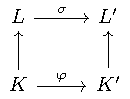
\includegraphics{./tikz/lemma_1_3_12.pdf}
\end{center}
\end{lemma}
\begin{proof}[was für die Prüfung!]\leavevmode\vspace*{\dimexpr-\baselineskip+2\lineskip}
	\begin{itemize}
		\item $f(\alpha) = 0$ $\Rightarrow$ $0 = \sigma(0) = \sigma\big(f(\alpha)\big) = \sigma\big(\sum_{i=0}^n a_i \alpha^i\big) = \sum_{i=0}^n \varphi(a_i)\sigma(\alpha)^i = f^{\varphi}\big(\sigma(\alpha)\big)$
		\item Eindeutigkeit klar, da $L=K(\alpha)$
		\item Existenz: Betrachte 
		\begin{align*}
			\eta\colon&
			\left\lbrace\begin{array}{@{}l@{\;}c@{\;}l}
				K[X] &\to& L\\
				g &\mapsto& g(\alpha)
			\end{array}\right.&
			\psi\colon&
			\left\lbrace\begin{array}{@{}l@{\;}c@{\;}l}
				K[X] &\to& L'\\
				g &\mapsto& g^{\varphi}(\beta) 
			\end{array}\right.
		\end{align*}
		Beide sind Homomorphismen nach der universellen Eigenschaft.
		(Bemerke: $\eta$ surjektiv: $\eta_{\mid K} = \id \to K \subset \Image(\eta)$ mit $\eta(X) = \alpha \to \alpha \in \Image(\eta)$)\\
		Aus $\Ker(\eta)=(f)$ folgt der Isomorphismus $\bar{\eta}\colon \lnkset{K[X]}{(f)} \xrightarrow{\cong}L$ und\\
		$f \in \Ker(\psi) \Rightarrow \Ker(\psi) = (f)$ liefert Homomorphismus $\bar{\psi}\colon \lnkset{K[X]}{(f)} \to L'$\\
		$\sigma:= \bar{\psi}\circ \bar{\eta}^{-1}\colon L \to L'$ ist eine Fortsetzung von $\phi$ und
		\begin{align*}
			\sigma(\alpha) = \bar{\psi}(X+(f)) = \beta
		\end{align*}
	\end{itemize}
\end{proof}
\begin{proposition}
	\proplbl{1_3_13}
	Der Zerfällungskörper von $f$ ist eindeutig bestimmt bis auf $K$-Isomorphie.
\end{proposition}
\begin{proof} Für den Beweis betrachte erst folgende Aussage.
	\begin{adjustwidth}{1em}{-6pt}
	\begin{underlinedenvironment}[Behauptung]
		Ist $\varphi\colon K \to K'$ ein Isomorphismus, $L$ ein Zerfällungskörper und $L'$ ein Zerfällungskörper von $f^{\varphi}$, so setzt sich $\varphi$ zu einem Isomorphismus $L \to L'$ fort.
	\end{underlinedenvironment}
	\vspace*{-\baselineskip}
	\begin{proof}\NoEndMark
			Induktion nach $n = \deg(f)$:
			\vspace*{-4\lineskip}
			\begin{itemize}[leftmargin=4.5em,itemsep=-2\lineskip] %TODO maybe use enum here without label?
				\item[$n=1$:] $L = K \xrightarrow[\varphi]{\cong} K' = L'$ \checkmark
				\item[$n>1$:] Schreibe $f = cg_1\cdots g_r$ mit $g_i \in K[X]$ normiert und irreduzibel, $c \in K^{\times}$\\[-0.8mm]
				\begin{tabularx}{\linewidth}{@{\hspace{0.5em}}r@{$\;\;$}X}
					$\Rightarrow$ & $f^{\varphi} = c^{\varphi}g_1^{\varphi}\cdots g_r^{\varphi}$ mit $c^{\varphi}\in (K')^{\varphi}$ und $g_i^{\varphi}\in K' [X]$ normiert und irreduzibel (weil $\varphi$ Isomorphismus ist). Sei $\alpha_1 \in L$ mit $g_1 (\alpha_1) = 0$, $\alpha'_1 \in L'$ mit $g_1^{\varphi}(\alpha'_1) = 0$\\
					$\xRightarrow{\propref{1_3_12}}$ & \begin{minipage}[t]{\linewidth}
						$\varphi$ setzt man zu einem Isomorphismus
					\[
						\sigma\colon K_1 := K(\alpha_1) \to K' (\alpha'_1) \quad \mit \sigma(\alpha_1) = \alpha'_1
					\]
					fort.
					\end{minipage} \\[16mm]
					\multicolumn{2}{l}{Schreibe $f=(x - \alpha_1)\cdot f_1$ mit $f_1 \in K_1 [X]$} \\[-2mm]
					$\Rightarrow$ & $f^{\varphi} = \big(x - \underbrace{\sigma(\alpha_1)}_{\alpha'_1}\big)\cdot f_1^{\sigma}$ mit $f_1^{\sigma}\in K'_1 [X]$.\\[-2mm]
					&$L$ ist Zerfällungskörper von $f_1$, $L'$ ist Zerfällungskörper von $f_1^{\sigma}$\\
					$\Rightarrow$ &  $\sigma$ setzt sich fort zu einem Isomorphismus $L \to L'$\hfill\csname\InTheoType Symbol\endcsname
				\end{tabularx}
			\end{itemize}
		\end{proof}
		\end{adjustwidth}
		Die Behauptung im Fall $\varphi = \id_K$ ist genau die Aussage von \propref{1_3_13}.
\end{proof}
\begin{remark}
	Ist $M\mid K$ eine Erweiterung, die einem Zerfällungskörper $L$ von $f$ enthält, dann ist dieser nicht nur bis auf die Isomorphie sondern als Teilkörper eindeutig bestimmt: $L = K(\alpha_1, \dots, \alpha_n)$, wobei $\alpha_1, \dots, \alpha_n$ genau die $n$ Nullstellen von $f$ in $M$ sind.
\end{remark}
\section{Der Algebraische Abschluss}
Sei $L\mid K$ eine Körpererweiterung.
\section{Separable Polynome}
Sei $K$ ein Körper, $f \in K[X]$, $n = \deg(f)$.
\begin{definition}
	Sei $a \in K$.
	\begin{enumerate}[label={(\arabic*)}]
		\item $\mu(f,a) := v_{x-a}(f) := \sup \set{k \in \N_0 : (x-a)^k \mid f} \in \N_0 \cup \set{\infty}$ die \begriff{Vielfachheit} der Nullstelle $a$ von $f$
		\item Nullstelle $a$ von $f$ ist \begriff{einfach} :$\Leftrightarrow$ $\mu(f,a) = 1$
		\item $f$ ist \begriff{separabel} :$\Leftrightarrow$ jede Nullstelle $a\in\bar K$ von $f\in\bar K[X]$ ist einfach.
	\end{enumerate}
\end{definition}
\begin{remark}
	\begin{enumerate}[label={(\alph*)}]
		\item Ist $L\mid K$ eine Körpererweiterung und $g\in K[X]$, so gilt \begin{flalign*}
			\qquad & f\mid g\;\text{in}\; K[X]\quad\Leftrightarrow\quad f\mid g\;\text{in}\; L[X]
		\end{flalign*}
		Insbesondere ist die Nullstelle $\mu_K(f,a) = \mu_L(f,a)$. Wir können deshalb von der Vielfachheit der Nullstelle von $f$ sprechen.
		\item \label{1_6_2_b} $\displaystyle\#\{a\in K\mid f(a) = 0\} \le \sum_{a\in K} \mu(f,a) \le \sum_{a\in \bar K} \mu(f,a) = \deg(f)$, falls ($f\neq 0$)
		\item Aus \ref{1_6_2_b} folgt insbesondere:\\
		\begin{tabularx}{\linewidth}{XcX}
			\hfill$f$ ist separabel & $\Leftrightarrow$ & $f$ hat genau $\deg(f)$ paarweise verschiedene Nullstellen in $\bar K$
		\end{tabularx}
	\end{enumerate}
\end{remark}
\begin{definition}
	Die \begriff{formale Ableitung} von $f = \sum_{i=1}^n a_i X^{i-1}$ ist \begin{flalign*}
		\qquad &f' := \frac{\d}{\d x} f(x) := \sum_{i=1} i a_i X^{i-1} &
	\end{flalign*}
\end{definition}
\begin{lemma}
	Für $f,g \in K[X], a,b \in K$ gelten\begin{enumerate}[label={(\alph*)}]
		\item $(af + bg)' = a f' + b g'$ (Linearität)
		\item $(fg)' = f'g + fg'$ (Produktregel)
		\item $(f(g(x)))' = f'(g(x))\cdot g'(x)$ (Kettenregel)
	\end{enumerate}
\end{lemma}
\begin{proof}
	Übung.
\end{proof}
\begin{lemma}
	\proplbl{1_6_5}
	Sei $f \neq 0$. Für $a \in K$ gilt
	\begin{flalign*}
		\qquad&\mu(f' , a) \ge \mu(f,a) - 1&
	\end{flalign*}
	mit Gleichheit genau dann, wenn $\chara(K) \nmid \mu(f,a)$.
\end{lemma}
\begin{proof}
	Schreibe $f = (X-a)^k \cdot g$, $k = \mu(f,a)$
	\begin{itemize}[topsep=-.5em,left=3.5em]
		\item[$k=0$:] $\mu(f', a) \ge 0 > -1$ und $\chara(K) \mid 0$
		\item[$k>0$:] $f' = k(X-a)^{k-1}g + (X-a)^k \cdot g'$ $\implies \mu(f',a) \ge k$, sowie 
		
		\vspace*{-2pt}
		\begin{tabular}{@{}>{$}r<{$}>{$}c<{$}>{$}l<{$}}
			\mu(f', a) \ge k & \Leftrightarrow & (X-a)^k \mid k(X-a)^{k-1}\cdot g \\
							 & \Leftrightarrow & X-a \mid k\cdot g \\
							 & \Leftrightarrow & X-a\mid k \\
							 & \Leftrightarrow & k=0\;\text{in}\; K\\
							 & \Leftrightarrow & \chara(K) \mid k
		\end{tabular}
	\end{itemize}
\end{proof}

\begin{proposition}
	Sei $f\neq 0$. Dann gilt:
	
	\begin{tabular}{@{$\qquad$}rcl}
		$f$ separabel & $\Leftrightarrow$ & $\ggT(f,f') = 1$
	\end{tabular}
\end{proposition}

\begin{proof}\leavevmode\vspace*{\dimexpr-\baselineskip+2\lineskip}
	\begin{itemize}
		\item[($\Rightarrow$)] $f$ separabel \\[-0.2em]
			\begin{tabular}[t]{@{}>{$}r<{$}@{$\;$}l}
			\Rightarrow & $f = c\cdot\prod_{i=1}^{n}(X-a_i)$ mit $c\in K$, $a_1$, $\dots$, $a_n\in \bar K$ paarweise verschieden und $\mu(f,a_i) = 1$ \\
			\xRightarrow[\chara(K)\nmid 1]{\propref{1_6_5}} & $\mu(f',a_i) = 0$ $\forall i$\\
			\Rightarrow & $\displaystyle\ggT(f,f') = \prod_{a\in\bar K} (X-a)^{\min\{ \mu(f,a), \mu(f',a) \}} = 1$
		\end{tabular}
		\item[($\Leftarrow$)] $f$ nicht separabel $\Rightarrow$ $\exists a\in\bar K$ mit $\mu(f,a)\ge 2$ $\xRightarrow{\propref{1_6_5}}$ $\mu(f',a)\ge 1$.
		
		Mit $g = \MinPol(a\mid K)$ gilt: $g\mid f$ $\Rightarrow$ $\ggT(f,f') \neq 1$
	\end{itemize}
\end{proof}

\begin{lemma}
	$f' = 0$ $\Leftrightarrow$ $\exists g\in K[X]$ mit $F(X) = g(X^p)$ und $p=\chara(K)$.
\end{lemma}
\begin{proof}
	Ist $f = \sum_{i=1}^{n} a_iX^i$ $\Rightarrow$ $f' = \sum_{i=1}^{n}i a_{i-1}X^{i-1}$ und \\[-0.3em]
	\begin{tabular}{@{}r>{$}c<{$}l}
		$f' = 0$	& \Leftrightarrow & $i a_i = 0$ in $K$ $\forall i$\\
					& \Leftrightarrow & $\forall i$: $i = 0$ in $K$ oder $a_i = 0$ \\
					& \Leftrightarrow & $f = a_0 + a_p X^p + \dots + a_{pm} X^{pm} = g(X^p)$ mit $g = a_0 + a_p X + \dots + a_{pm} X^m$
	\end{tabular}
\end{proof}

%TODO
\begin{conclusion}
	Sei $f$ irreduzibel
	\begin{enumerate}[label={(\alph*)}]
		\item Ist $\chara(K) = 0$, so ist $f$ separabel
		\item Ist $\chara(K) = p>0$, so sind äquivalent
		\begin{enumerate}[label={(\arabic*)}]
			\item $f$ ist inseparabel
			\item $f' = 0$
			\item $f(X) = g(X^p)$ für ein $g \in K[X]$
		\end{enumerate}
	\end{enumerate}
\end{conclusion}
\begin{proof}
	$f$ irreduzibel $\implies \underbrace{\ggT(f,f') \sim 1}_{\iff f \text{ sep}} \oder \underbrace{\ggT(f,f') \sim f}_{\iff f \text{ sep.}}$. (Nutze 6.6 für die $\iff$) Da $\deg(f') = \deg(f)$ ist
	\[
		f \mid f' \iff f' = 0 \iff f(x) = g(x^p). \text{ für ein }g
	\]
	Im Fall $\chara(K) = 0$ tritt dieser Fall nicht ein.
\end{proof}
\begin{definition}[vollkommen]
	$K$ ist \begriff{vollkommen} $\iff$ jedes irreduzibel $f \in K[X]$ ist separabel.
\end{definition}
\begin{example}
	\begin{enumerate}
		\item $\chara(K) = 0 \implies K$ ist vollkommen
		\item $K = \bar{K} \implies K$ ist vollkommen
		\item $K = \F_p (t)$ ist nicht vollkommen:
		\begin{align*}
			f = X^p - t \in K[X] \text{ ist irreduzibel}\\
			f' = X^{p-1} = 0 \implies f \text{ nicht seperabel.}
		\end{align*}
		Tatsächlich hat $f$ nur eine Nullstelle in $\bar{K}$:
		\begin{align*}
			f = X^p - t \overset{V1}{=} (X - t^{\frac{1}{t}})^p
		\end{align*}
	\end{enumerate}
\end{example}
\begin{definition}[title]
	Sei $\chara(K) = p > 0$.
	\begin{enumerate}
		\item \begin{align*}
		\varphi_p : \begin{cases}
		K &\to K\\
		x &\mapsto x^p 
		\end{cases}
		\end{align*}
		\person{Frobenius}-Endomorphismus von $K$
		\item $K^p = \Image(\varphi_p) = \set{a^p : a \in K}$
	\end{enumerate}
\end{definition}
\begin{proposition}
	Sei $\chara(K) = p > 0$. Dann ist $\varphi_p \in \End(K): =\Hom(K,K)$
\end{proposition}
\begin{proof}
	Für $a, b \in K$ ist
	\begin{itemize}
		\item $\varphi_p = (ab)^p = a^p \cdot b^p = \varphi_p (a) \cdot \varphi_p(b)$
		\item $\varphi_p(a+b) = (a+b)^p = \sum_{i=0}^p\binom{p}{i} a^i b^{p-i} = b^p + a^p = \varphi_p(a) + \varphi_p(b)$, da $p \mid \binom{p}{i}$ für $i = 1, \dots, p-1$ (V1).
		\item $\varphi_p(1) = 1^p = 1$
	\end{itemize}
\end{proof}
\begin{remark}
	\begin{enumerate}
		\item Da $\varphi_p \in \End(K) $ ist $K^p$ ein Teilkörper von $K$ und $\varphi_p$ ist injektiv.
		\item Insbesondere gibt es zu jedem $a \in K$ ein eindeutig bestimmtes $a^{\frac{1}{p}} \in \bar{K}$ mit
		\[
			\varphi_p(a^{\frac{1}{p}}) = (a^{\frac{1}{p}})^p = a
		\]
		\item Für $a \in \F \cong \F_p$ ist $\varphi_p(a) = a$. (z.B. $\varphi_p(1) = 1$ oder kleiner Satz von \person{Fermat})
	\end{enumerate}
\end{remark}
\begin{lemma}
	Sei $\chara(K) = p > 0, a \in K \setminus K^p$. Dann ist $f = X^p -a$ irreduzibel und inseparabel
\end{lemma}
\begin{proof}
	Sei $\alpha \in \bar{K}$ mit $f(\alpha) = 0, g= \MinPol(\alpha \mid K)$\\
	$\implies g \mid f = X^p -a = (X-\alpha)^p$\\
	$\implies g \equiv (X - \alpha)^k \mit k \le p$. $a \notin K^p \implies \alpha \notin K \implies k >1$\\
	$\implies g$ ist inseperabel\\
	$\xRightarrow{g \text{ irred.}} g(x) = h(x^p)$ für ein $h$\\
	$\implies k = p \implies f = g$ irreduzibel 
\end{proof}

\part*{Anhang}
\addcontentsline{toc}{part}{Anhang}
\appendix

%\printglossary[type=\acronymtype]

\printindex

\end{document}
